\begin{figure}[t]
\centering
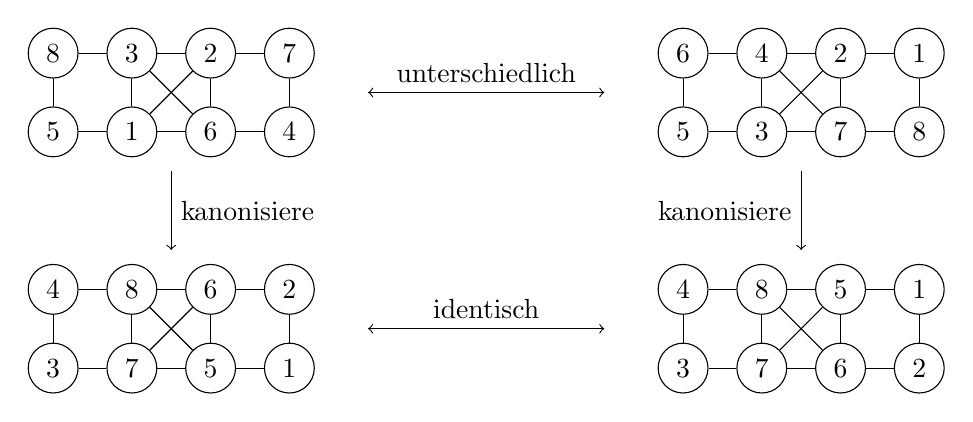
\begin{tikzpicture}
  \tikzstyle{node}=[circle,draw, minimum width=18pt, inner sep=0pt, fill=white]

  \node[node] (a1) at (0, 4) {$8$};
  \node[node] (a2) at (1, 4) {$3$};
  \node[node] (a3) at (2, 4) {$2$};
  \node[node] (a4) at (3, 4) {$7$};
  \node[node] (a5) at (0, 3) {$5$};
  \node[node] (a6) at (1, 3) {$1$};
  \node[node] (a7) at (2, 3) {$6$};
  \node[node] (a8) at (3, 3) {$4$};

  \path (a1) edge (a2);
  \path (a1) edge (a5);
  \path (a2) edge (a3);
  \path (a2) edge (a6);
  \path (a2) edge (a7);
  \path (a3) edge (a4);
  \path (a3) edge (a6);
  \path (a3) edge (a7);
  \path (a4) edge (a8);
  \path (a5) edge (a6);
  \path (a6) edge (a7);
  \path (a7) edge (a8);

  \node[node] (b1) at (0, 1) {$4$};
  \node[node] (b2) at (1, 1) {$8$};
  \node[node] (b3) at (2, 1) {$6$};
  \node[node] (b4) at (3, 1) {$2$};
  \node[node] (b5) at (0, 0) {$3$};
  \node[node] (b6) at (1, 0) {$7$};
  \node[node] (b7) at (2, 0) {$5$};
  \node[node] (b8) at (3, 0) {$1$};

  \path (b1) edge (b2);
  \path (b1) edge (b5);
  \path (b2) edge (b3);
  \path (b2) edge (b6);
  \path (b2) edge (b7);
  \path (b3) edge (b4);
  \path (b3) edge (b6);
  \path (b3) edge (b7);
  \path (b4) edge (b8);
  \path (b5) edge (b6);
  \path (b6) edge (b7);
  \path (b7) edge (b8);

  \node[node] (c1) at (8,  4) {$6$};
  \node[node] (c2) at (9,  4) {$4$};
  \node[node] (c3) at (10, 4) {$2$};
  \node[node] (c4) at (11, 4) {$1$};
  \node[node] (c5) at (8,  3) {$5$};
  \node[node] (c6) at (9,  3) {$3$};
  \node[node] (c7) at (10, 3) {$7$};
  \node[node] (c8) at (11, 3) {$8$};

  \path (c1) edge (c2);
  \path (c1) edge (c5);
  \path (c2) edge (c3);
  \path (c2) edge (c6);
  \path (c2) edge (c7);
  \path (c3) edge (c4);
  \path (c3) edge (c6);
  \path (c3) edge (c7);
  \path (c4) edge (c8);
  \path (c5) edge (c6);
  \path (c6) edge (c7);
  \path (c7) edge (c8);

  \node[node] (d1) at (8,  1) {$4$};
  \node[node] (d2) at (9,  1) {$8$};
  \node[node] (d3) at (10, 1) {$5$};
  \node[node] (d4) at (11, 1) {$1$};
  \node[node] (d5) at (8,  0) {$3$};
  \node[node] (d6) at (9,  0) {$7$};
  \node[node] (d7) at (10, 0) {$6$};
  \node[node] (d8) at (11, 0) {$2$};

  \path (d1) edge (d2);
  \path (d1) edge (d5);
  \path (d2) edge (d3);
  \path (d2) edge (d6);
  \path (d2) edge (d7);
  \path (d3) edge (d4);
  \path (d3) edge (d6);
  \path (d3) edge (d7);
  \path (d4) edge (d8);
  \path (d5) edge (d6);
  \path (d6) edge (d7);
  \path (d7) edge (d8);

  \draw[<->] (4,   3.5) -- node[above] {unterschiedlich} (7,   3.5);
  \draw[<->] (4,   0.5) -- node[above] {identisch}       (7,   0.5);
  \draw[->]  (1.5, 2.5) -- node[right] {kanonisiere}     (1.5, 1.5);
  \draw[->]  (9.5, 2.5) -- node[left]  {kanonisiere}     (9.5, 1.5);

\end{tikzpicture}
\caption[Kanonische Ordnung]{Illustration zweier isomorpher Graphen (oben), die jedoch nicht identisch sind (\zB{} sind die Knoten $1$ und $5$ im linken Graphen adjazent, aber nicht im rechten).
Der Prozess der Kanonisierung sorgt dafür, dass zwei Graphen eine identische Knotenabbildung erhalten, falls sie isomorph zueinander sind (unten).
Die Kanten der Graphen verweisen jeweils auf die gleichen Indizes, auch wenn sich die Darstellung \bzw{} Position der Knoten unterscheidet.}
\label{fig:kanonische_ordnung}
\end{figure}
